% !TeX program = xelatex
% !TeX encoding = UTF-8
% ...existing code...
\documentclass[a4paper]{article}

\usepackage[UTF8]{ctex}
\usepackage[a4paper,margin=1in]{geometry}
\usepackage{graphicx}
\usepackage{listings}
% \usepackage{listings-rust}
\usepackage{longtable}
\usepackage{booktabs}
\usepackage{hyperref}
\usepackage{fancyhdr}
\usepackage{lastpage}
\usepackage{color}
\usepackage{indentfirst}        % 首段缩进
\setlength{\parindent}{2em}     % 缩进2字符
\usepackage{zhnumber}           % 中文编号
\usepackage[dvipsnames,table,xcdraw]{xcolor}
\usepackage{adjustbox}
\usepackage{subcaption}
\usepackage{float}
\usepackage{amsmath}
\usepackage{amssymb}
\usepackage[many]{tcolorbox}
% \newfontfamily{\enfont}{Arial}  % 定义英文字体
\usepackage{enumitem}
\usepackage{xeCJK}
\usepackage[T1]{fontenc}
\usepackage{lmodern}
\usepackage{inconsolata} % 使用更美观的等宽字体 Inconsolata
\usepackage{multirow} % 用于表格中的多行合并
\usepackage{tikz} % 添加 TikZ 宏包用于绘制流程图
\usetikzlibrary{positioning} % 添加定位库以支持 'of' 语法

% 全局设置（影响所有级别）
\setlist[itemize]{
    itemsep=2pt,
    topsep=4pt,
    parsep=1pt,
    leftmargin=3em
}

% 仅设置第一级（最高级）
\setlist[itemize,1]{
    label=\textcolor{orange}{$\blacktriangleright$},
    font=\color{blue!80!black}\small\bfseries,
    before={\color{blue!80!black}\small\bfseries}
}

% 重置第二级及更深级别（恢复默认样式）
\setlist[itemize,2]{
    label={\normalfont\textbullet},
    font=\normalfont\normalsize\color{black},
    before={\color{black}},
    leftmargin=*
}
\setlist[itemize,3]{
    label={\normalfont$\circ$},
    font=\normalfont\normalsize,
    before={},
    leftmargin=*
}


% 定义可分页的引用环境
\newtcolorbox[auto counter]{myquote}[1][]{
    % breakable,                     % 允许跨页分断
    % enhanced jigsaw,               % 优化分页处的边框
    colback=gray!5,                % 背景色
    colframe=gray!30,              % 边框色
    left=5mm, right=5mm,           % 左右内边距
    top=3mm, bottom=3mm,           % 上下内边距
    width=0.85\textwidth,         % 宽度
    center,                     % 居中
    arc=0mm,                       % 直角边框
    boxrule=0.5pt,                 % 边框线宽
    fontupper=\small\linespread{1.1}\selectfont, % 行距微调（1.1倍）
    % fontupper=\sffamily\linespread{1.05}\selectfont, % 无衬线 + 紧凑行距
    before upper={\parindent2em\color{black!40!blue}\itshape\small\kaishu}, % 深蓝色文本
    #1 % 允许额外参数
}

%\newcommand{\college}{中山大学计算机学院}
\newcommand{\projname}{计算机网络实验|实验六}
\newcommand{\reporttitle}{跨交换机实现VLAN}
\newcommand{\groupno}{第一组}
\newcommand{\authorname}{欧阳易芃、马福泉、刘昊、彭怡萱}
\newcommand{\major}{计算机科学与技术}
\newcommand{\adviser}{谢逸}
\newcommand{\startdate}{2025年11月10日}
\newcommand{\labenddate}{2025年11月23日}
\newcommand{\labroom}{实验D402}

\pagestyle{fancy} % 使用 fancyhdr 风格
\fancyhf{}      % 清空默认的页眉页脚

% 设置页眉
\fancyhead[L]{\kaishu \projname}      % 左侧页眉显示项目名称
\fancyhead[C]{\kaishu \reporttitle}    % 中间页眉显示报告标题
\fancyhead[R]{\kaishu \authorname} % 右侧页眉显示作者姓名

% 设置页脚
\fancyfoot[C]{第 \thepage 页，共 \pageref{LastPage} 页} % 中间页脚显示页码

% 去除页眉页脚与正文之间的分隔线
\renewcommand{\headrulewidth}{0.4pt}
\renewcommand{\footrulewidth}{0pt}

% 设置文档背景颜色
\definecolor{mybgcolor}{RGB}{0, 0, 0} % 定义背景颜色
\definecolor{NavyBlue}{RGB}{0,0,128} % 添加颜色定义



% 全局设置lstlisting的样式
\lstset{
    language=C, % 设置默认语言
    basicstyle=\footnotesize\ttfamily, % 设置字体族
    breaklines=true, % 自动换行
    keywordstyle=\bfseries\color{blue}, % 设置关键字为粗体，颜色为蓝色
    morekeywords={}, % 设置更多的关键字，用逗号分隔
    emph={}, % 指定强调词，如果有多个，用逗号隔开
    emphstyle=\bfseries\color{Rhodamine},
    commentstyle=\itshape\color{green!50!black},
    stringstyle=\bfseries\color{PineGreen!90!black},
    columns=fullflexible,% 设置列宽
    numbers=left,
    numbersep=2em,
    numberstyle=\footnotesize\color{gray},
    frame=single,
    framesep=1em,
    showstringspaces=false,% % 不显示字符串中的空格
    keepspaces=true,
    backgroundcolor=\color{gray!5},
    % linewidth=0.8\linewidth, % 设置宽度为当前行宽的 80%
    xleftmargin=0.2\linewidth, % 左右边距自动调整
    xrightmargin=0.08\linewidth,
    % gobble=2, % 可选：移除代码前的缩进
    % postbreak=\mbox{\textcolor{red}{$\hookrightarrow$}\space}, % 可选：换行符样式
    captionpos=b, % 可选：标题位置
    aboveskip=1em, % 可选：上方间距
    belowskip=1em, % 可选：下方间距
}

\begin{document}


% 封面
\begin{titlepage}
    \centering
    
    
\includegraphics[width=10cm]{img/SYSULogo.png}

    \vspace{1em}
    %{\Large \college \par}
    \vspace{1em}
    {\Large \kaishu \projname \par}
    \vspace{3em}

    {\fontsize{40pt}{42pt}\kaishu \selectfont \boldmath \reporttitle\par}
    \vspace*{\fill}

    \begin{center}
    {\Large
    \makebox[5em][s]{小组编号}:\underline{\makebox[15em][c]{\kaishu \groupno}}\\[1em]
    \makebox[5em][s]{组员姓名}:\underline{\makebox[15em][c]{\kaishu 欧阳易芃、马福泉}}\\[0.5em]
    \makebox[5em][s]{} \underline{\makebox[15em][c]{\kaishu 刘昊、彭怡萱}}\\[1em]
    \makebox[5em][s]{专业}:\underline{\makebox[15em][c]{\kaishu \major}}\\[1em]
    \makebox[5em][s]{课程教师}:\underline{\makebox[15em][c]{\kaishu \adviser}}\\[1em]
    \makebox[5em][s]{起始日期}:\underline{\makebox[15em][c]{\kaishu \startdate}}\\[1em]
    \makebox[5em][s]{结束日期}:\underline{\makebox[15em][c]{\kaishu \labenddate}}\\[1em]
    \makebox[5em][s]{实验地点}:\underline{\makebox[15em][c]{\kaishu \labroom}}
    }
    \end{center}

    \vspace*{\fill}
\end{titlepage}

% 目录
\tableofcontents
\newpage

\section{实验目的}
\begin{itemize}
    \item 理解VLAN的基本概念及其在交换机中的实现方式。
    \item 掌握跨交换机实现VLAN的配置方法。
    \item 验证同一VLAN内主机可通信，不同VLAN间主机隔离的特性。
\end{itemize}

\section{实验原理}
\subsection{VLAN简介}
VLAN（Virtual Local Area Network）是一种将物理局域网划分为多个逻辑局域网的技术。通过VLAN，可以在同一台交换机或跨交换机的情况下，将不同端口划分为不同的广播域，从而实现网络流量的隔离和安全控制。

\subsection{交换机端口类型}
\begin{itemize}
    \item \textbf{Access端口}：用于连接主机，只能属于一个VLAN。
    \item \textbf{Trunk端口}：用于交换机之间互联，可以传输多个VLAN的数据帧，通过VLAN标签（Tag）区分不同VLAN。
\end{itemize}

\subsection{跨交换机VLAN通信原理}
当两台交换机之间需要传输多个VLAN的数据时，需将连接端口设置为Trunk模式，并在数据帧中插入VLAN标签。接收方交换机根据标签将数据帧转发到相应VLAN的端口。


\subsubsection{VLAN标签}
要使设备能够分辨不同VLAN的报文，需要在报文中添加标识VLAN信息的字段。IEEE 802.1Q协议规定，在以太网数据帧的目的MAC地址和源MAC地址字段之后、协议类型字段之前加入4个字节的VLAN标签(VLAN tag)，用以标识VLAN信息。

\subsubsection{VLAN帧格式}
\begin{figure}[H]
    \centering
    \adjustbox{
        max width=0.8\linewidth,
        max height=0.6\textheight,
        min width=1cm,
        min height=1cm,
        keepaspectratio
    }{
        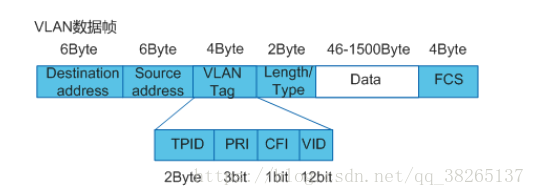
\includegraphics{img/vlan_tag.png}
    }
    \caption{VLAN帧格式}
\end{figure}


\section{实验环境}
\begin{itemize}
    \item 交换机A(S1)、交换机B(S2)
    \item PC1、PC2、PC3
    \item 管理软件：MobaXterm
\end{itemize}

\section{实验步骤与结果分析}

\subsection{步骤1：实验前测试}
\subsubsection{操作内容}
为三台主机配置IP地址：
\begin{lstlisting}[language=bash]
PC1：netsh interface ipv4 set address name="实验网" static 192.168.10.10 255.255.255.0
PC2：netsh interface ipv4 set address name="实验网" static 192.168.10.20 255.255.255.0
PC3：netsh interface ipv4 set address name="实验网" static 192.168.10.30 255.255.255.0
netsh interface ipv4 show interfaces （查看网络接口 IPv4 配置信息）
\end{lstlisting}
\begin{figure}[H]
    \centering
    % 第一张图片
    \begin{minipage}[t]{0.8\textwidth}
        \centering
        \adjustbox{
            max width=0.8\linewidth,
            max height=0.3\textheight,
            min width=1cm,
            min height=1cm,
            keepaspectratio
        }{
            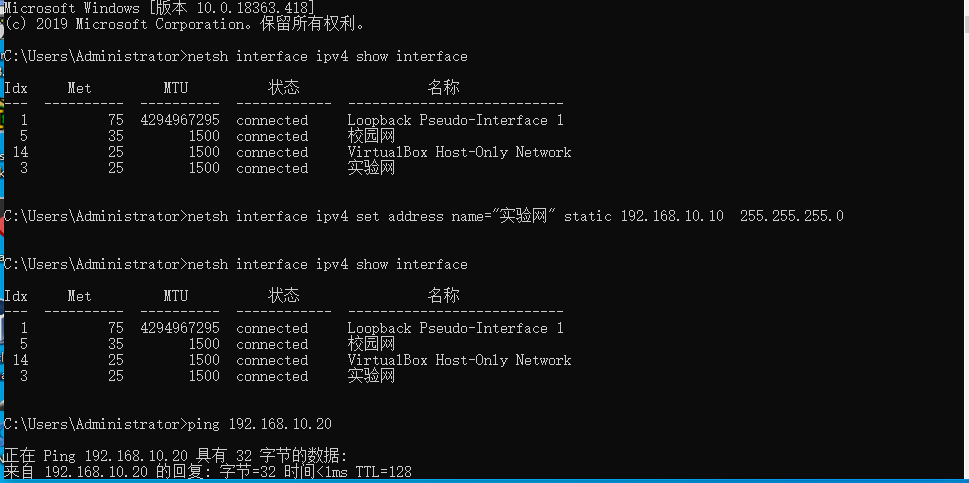
\includegraphics{img/pc1.png}
        }
        \subcaption{PC1配置}
        \label{fig:pc1-config}
    \end{minipage}
    
    \vspace{0.5em}
    
    % 第二张图片
    \begin{minipage}[t]{0.8\textwidth}
        \centering
        \adjustbox{
            max width=0.8\linewidth,
            max height=0.3\textheight,
            min width=1cm,
            min height=1cm,
            keepaspectratio
        }{
            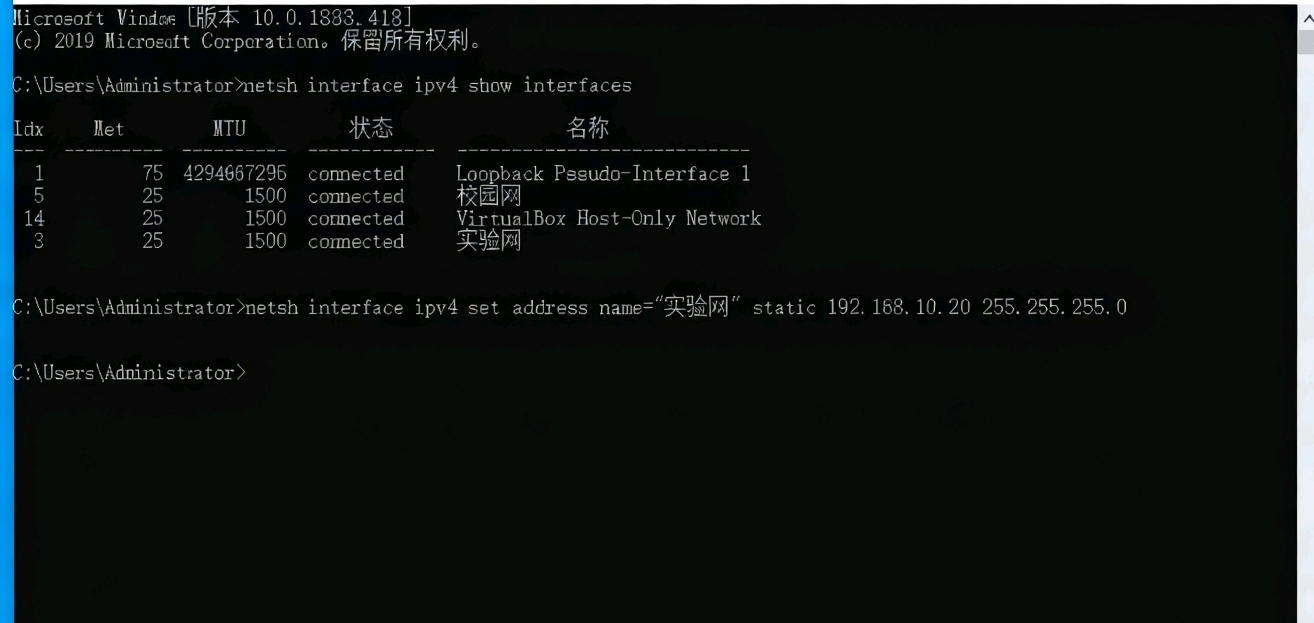
\includegraphics{img/pc2.jpg}
        }
        \subcaption{PC2配置}
        \label{fig:pc2-config}
    \end{minipage}
    
    \vspace{0.5em}
    
    % 第三张图片
    \begin{minipage}[t]{0.8\textwidth}
        \centering
        \adjustbox{
            max width=0.8\linewidth,
            max height=0.3\textheight,
            min width=1cm,
            min height=1cm,
            keepaspectratio
        }{
            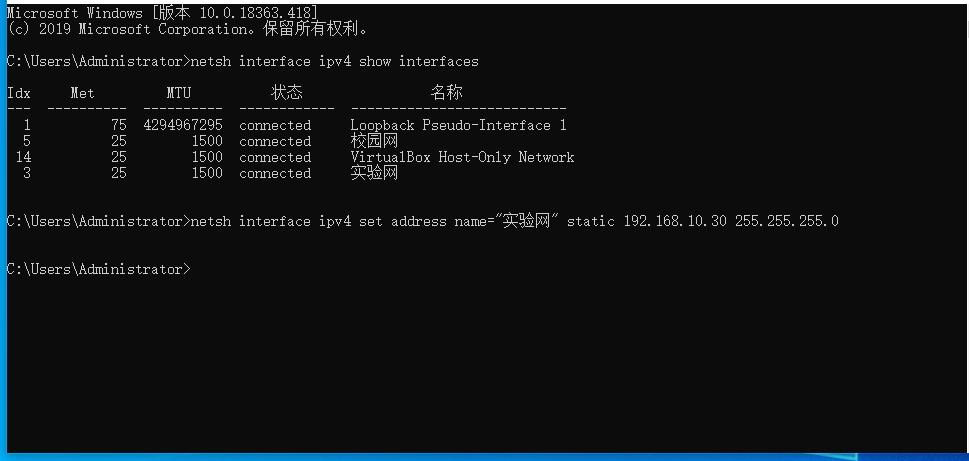
\includegraphics{img/pc3.png}
        }
        \subcaption{PC3配置}
        \label{fig:pc3-config}
    \end{minipage}
    \caption{三台主机配置}
    \label{fig:hosts-config}
\end{figure}

按照下面拓扑图连接PC1、PC2、PC3、交换机A和交换机B：
\begin{figure}[H]
    \centering
    \adjustbox{
        max width=0.8\linewidth,
        max height=0.6\textheight,
        min width=1cm,
        min height=1cm,
        keepaspectratio
    }{
        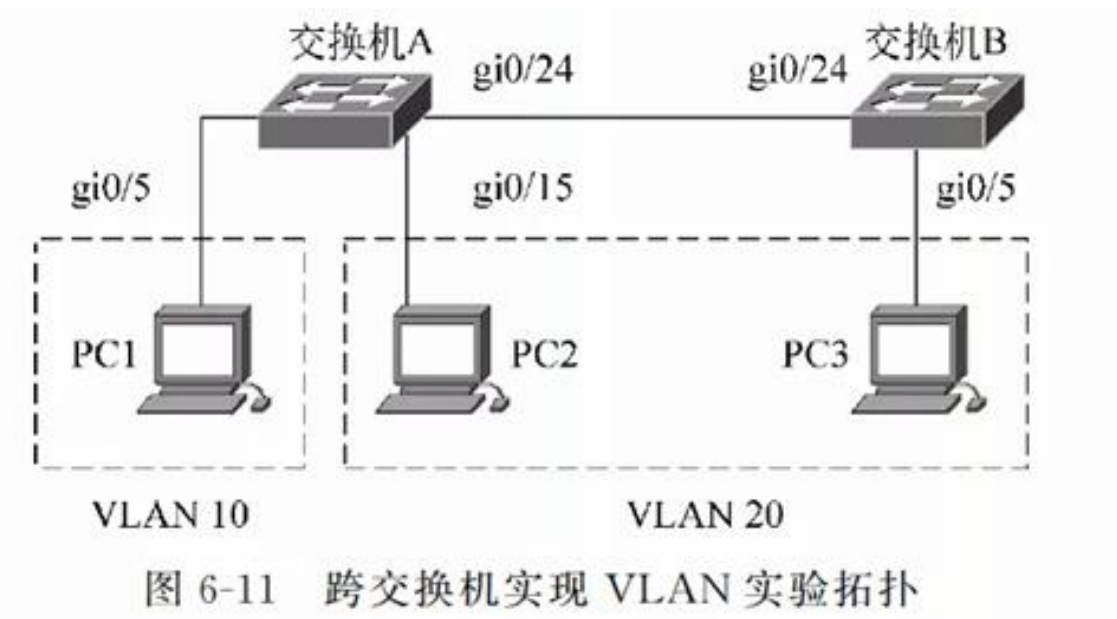
\includegraphics{img/tuopu.png}
    }
    \caption{实验拓扑图}
\end{figure}
\vspace{1em}
使用 \texttt{ping} 命令测试三台主机之间的连通性。
\begin{figure}[H]
    \centering
    % 第一张图片
    \begin{minipage}[t]{0.48\textwidth}
        \centering
        \adjustbox{
            max width=1.05\linewidth,
            max height=0.45\textheight,
            min width=1cm,
            min height=1cm,
            keepaspectratio
        }{
            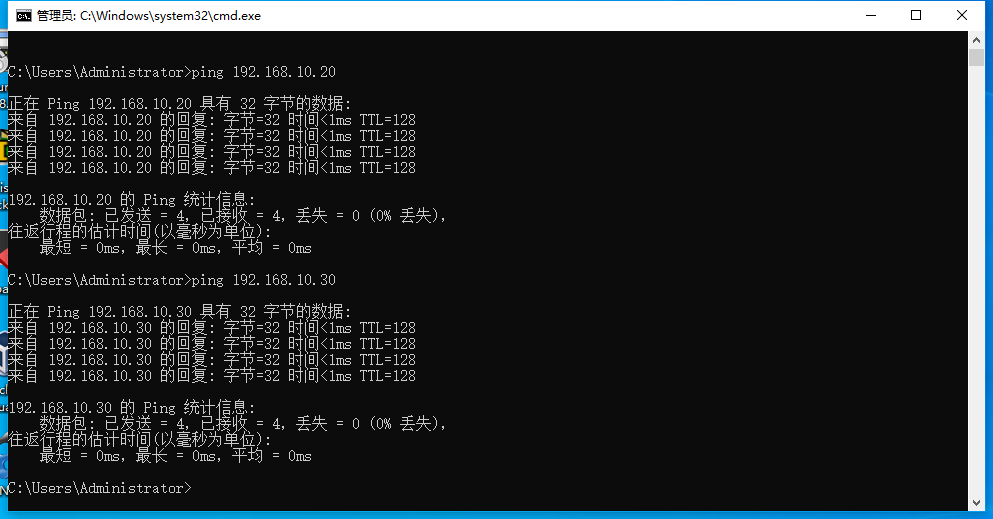
\includegraphics{img/pc1_ping.png}
        }
        \subcaption{PC1可以ping通PC2、PC3}
    \end{minipage}
    \hfill
    % 第二张图片
    \begin{minipage}[t]{0.48\textwidth}
        \centering
        \adjustbox{
            max width=1\linewidth,
            max height=0.45\textheight,
            min width=1cm,
            min height=1cm,
            keepaspectratio
        }{
            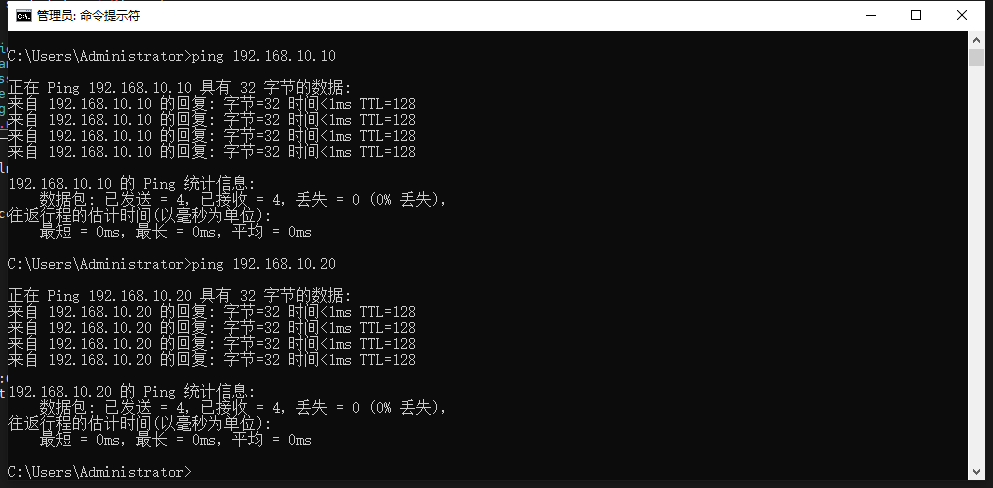
\includegraphics{img/pc3_ping.png}
        }
        \subcaption{PC3可以ping通PC1、PC2}
    \end{minipage}
    \caption{测试三台主机之间的连通性}
\end{figure}
在实验前，此时所有主机处于同一网段，且未划分VLAN，属于同一广播域，三台主机可以两两连通，符合预期。


\subsection{步骤2：在交换机A上创建VLAN 10并划分端口}
\subsubsection{操作内容}
在交换机 A 上创建 VLAN 10，并将 PC1 连接在交换机 A 上面的端口划分到 VLAN10 中
在 PC1 上进行操作：
\begin{lstlisting}[language=bash]
system-view
vlan 10
description sales
quit
interface GigabitEthernet 0/0/5
port link-type access
port default vlan 10
quit
\end{lstlisting}

\subsubsection{实验结果}
\begin{itemize}
    \item \texttt{display vlan 10} 显示端口5已加入VLAN 10。
    \begin{figure}[H]
    \centering
    \adjustbox{
        max width=0.8\linewidth,
        max height=0.6\textheight,
        min width=1cm,
        min height=1cm,
        keepaspectratio
    }{
        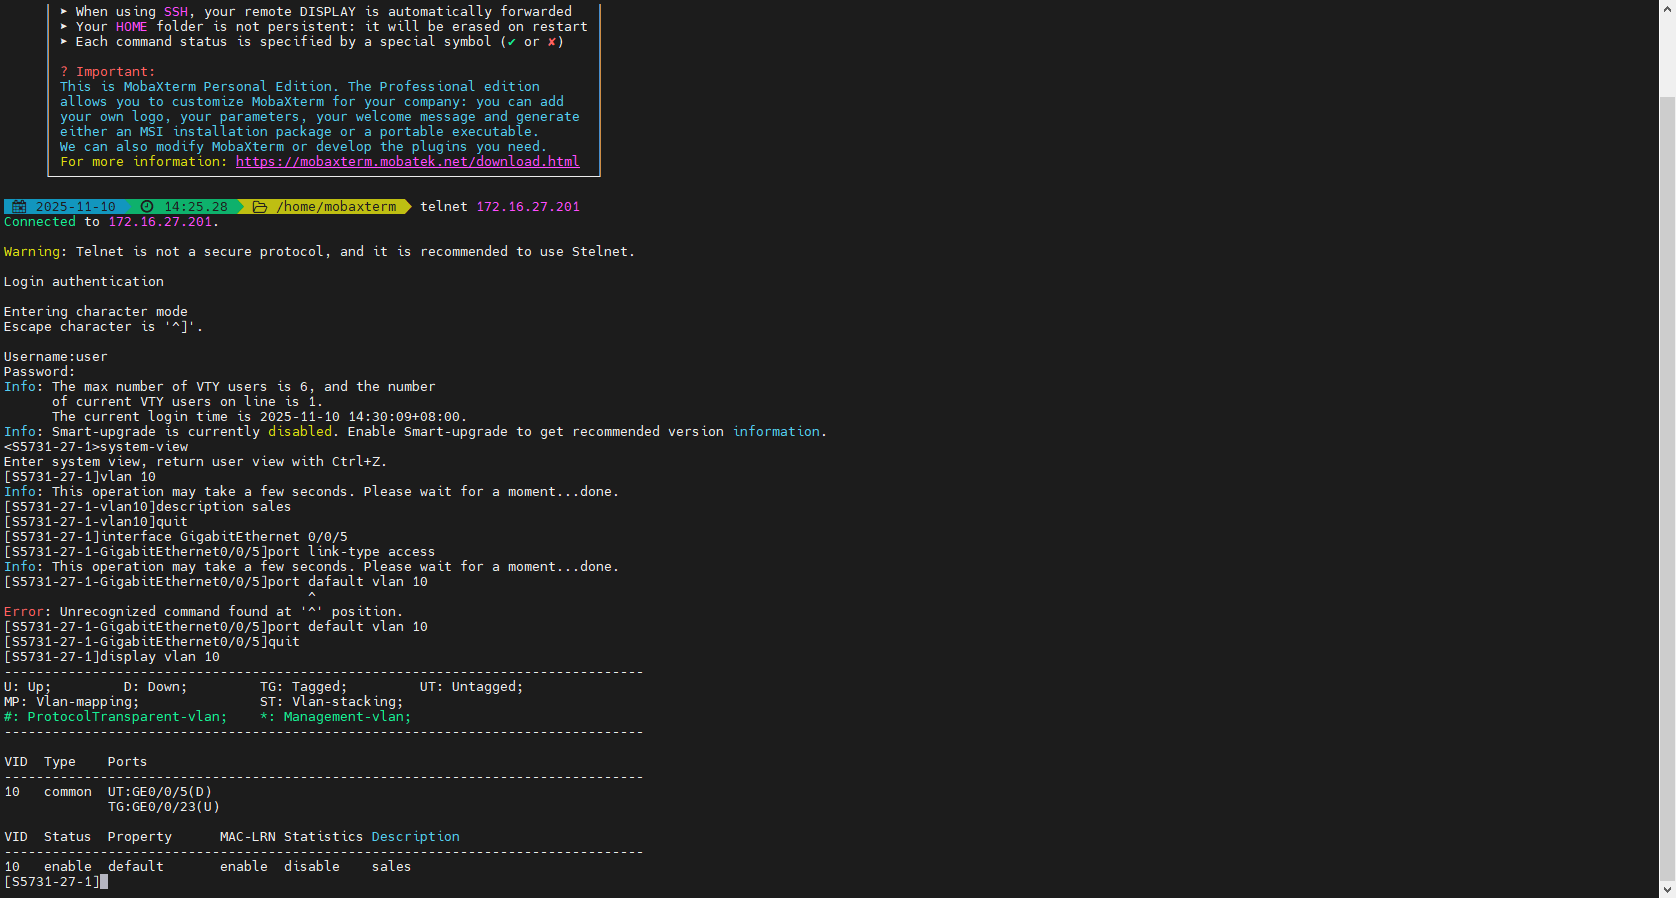
\includegraphics{img/vlan10.png}
    }
    \caption{成功划分交换机A的端口5到VLAN10}
    \end{figure}
    \item PC1与PC2、PC3之间无法 ping 通。
     \begin{figure}[H]
    \centering
    \adjustbox{
        max width=0.8\linewidth,
        max height=0.6\textheight,
        min width=1cm,
        min height=1cm,
        keepaspectratio
    }{
        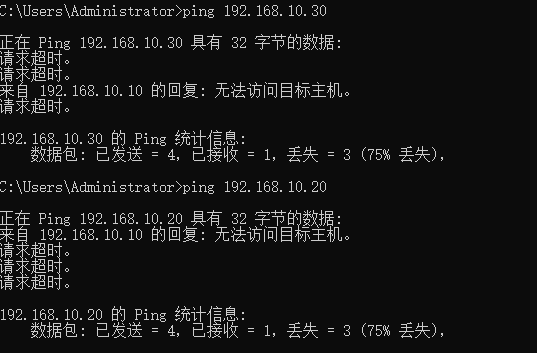
\includegraphics{img/pc1_ping(1).png}
    }
    \caption{pc1无法ping通pc2、pc3}
    \end{figure}
\end{itemize}

\subsubsection{原因分析}
PC1所在端口被划分到VLAN 10，而PC2和PC3仍在默认VLAN 1中，不同VLAN间无法直接通信。

\vspace{2em}
\subsection{步骤3：在交换机A上创建VLAN 20并划分端口}
\subsubsection{操作内容}
\begin{lstlisting}[language=bash]
vlan 20
description technical
quit
interface GigabitEthernet 0/0/15
port link-type access
port default vlan 20
quit
\end{lstlisting}

\subsubsection{实验结果}
\begin{itemize}
    \item \texttt{display vlan 20} 显示端口15已加入VLAN 20。
     \begin{figure}[H]
    \centering
    \adjustbox{
        max width=0.8\linewidth,
        max height=0.6\textheight,
        min width=1cm,
        min height=1cm,
        keepaspectratio
    }{
        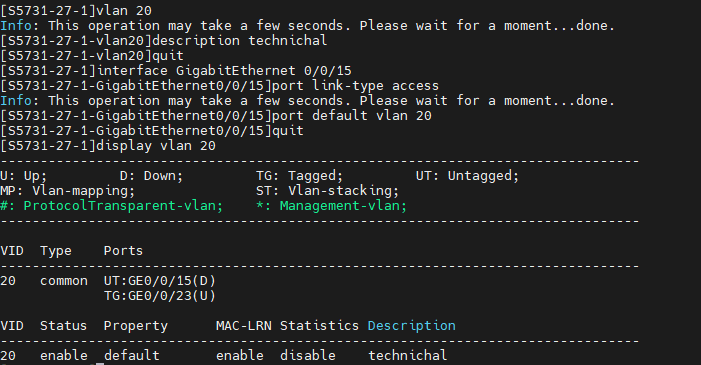
\includegraphics{img/vlan20.png}
    }
    \caption{成功划分交换机A的端口15到VLAN20}
    \end{figure}
    \item PC1、PC2、PC3之间均无法 ping 通。
    \begin{figure}[H]
    \centering
    % 第一张图片
    \begin{minipage}[t]{0.48\textwidth}
        \centering
        \adjustbox{
            max width=1.05\linewidth,
            max height=0.45\textheight,
            min width=1cm,
            min height=1cm,
            keepaspectratio
        }{
            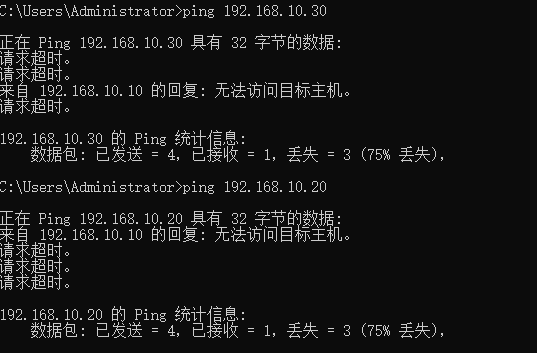
\includegraphics{img/pc1_ping(1).png}
        }
        \subcaption{PC1不可以ping通PC2、PC3}
    \end{minipage}
    \hfill
    % 第二张图片
    \begin{minipage}[t]{0.48\textwidth}
        \centering
        \adjustbox{
            max width=1\linewidth,
            max height=0.45\textheight,
            min width=1cm,
            min height=1cm,
            keepaspectratio
        }{
            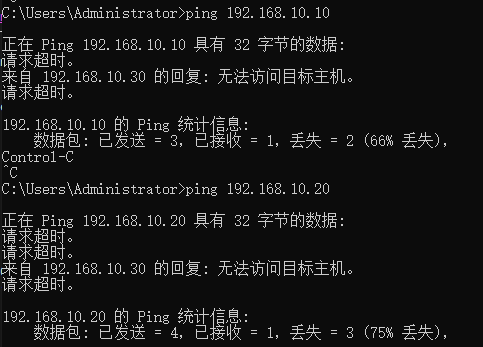
\includegraphics{img/pc3_ping(1).png}
        }
        \subcaption{PC3不可以ping通PC1、PC2}
    \end{minipage}
    \caption{测试三台主机之间的连通性}
\end{figure}
\end{itemize}
\subsubsection{原因分析}
PC1在VLAN 10，PC2在VLAN 20，PC3在VLAN 1，三者分属不同VLAN，无法通信。

\subsection{步骤4：配置交换机A与交换机B之间的Trunk链路}
\subsubsection{操作内容}
在交换机A上：
\begin{lstlisting}[language=bash]
interface GigabitEthernet 0/0/24
port link-type trunk
port trunk allow-pass vlan all
quit
\end{lstlisting}

\subsubsection{实验结果}
\begin{itemize}
    \item \texttt{display interface GigabitEthernet 0/0/24} 显示端口为Trunk模式。
    \begin{figure}[H]
    \centering
    \adjustbox{
        max width=0.8\linewidth,
        max height=0.6\textheight,
        min width=1cm,
        min height=1cm,
        keepaspectratio
    }{
        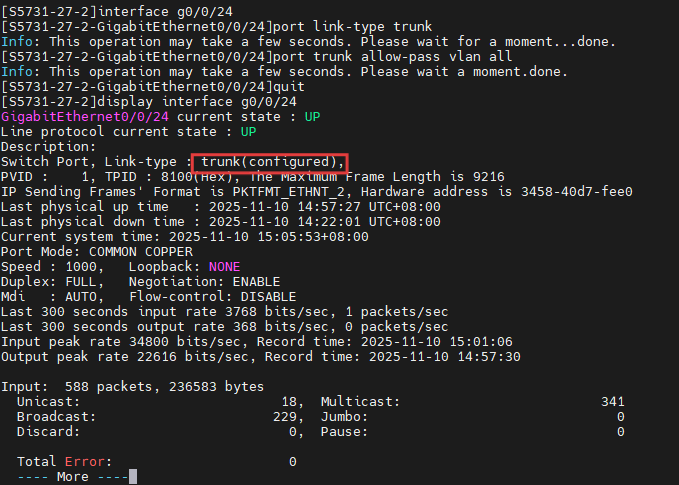
\includegraphics{img/trunk.png}
    }
    \caption{24号接口显示Link-type=trunk}
    \end{figure}
    \item PC1、PC2、PC3之间仍无法 ping 通。
     \begin{figure}[H]
    \centering
    % 第一张图片
    \begin{minipage}[t]{0.48\textwidth}
        \centering
        \adjustbox{
            max width=1.05\linewidth,
            max height=0.45\textheight,
            min width=1cm,
            min height=1cm,
            keepaspectratio
        }{
            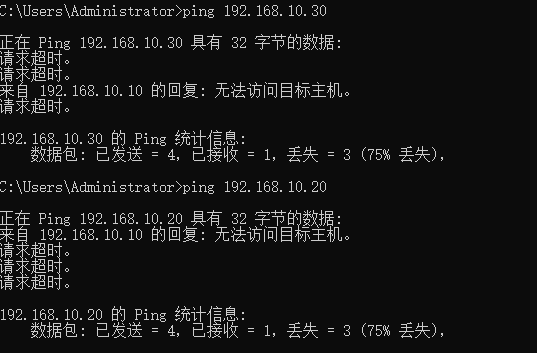
\includegraphics{img/pc1_ping(1).png}
        }
        \subcaption{PC1不可以ping通PC2、PC3}
    \end{minipage}
    \hfill
    % 第二张图片
    \begin{minipage}[t]{0.48\textwidth}
        \centering
        \adjustbox{
            max width=1\linewidth,
            max height=0.45\textheight,
            min width=1cm,
            min height=1cm,
            keepaspectratio
        }{
            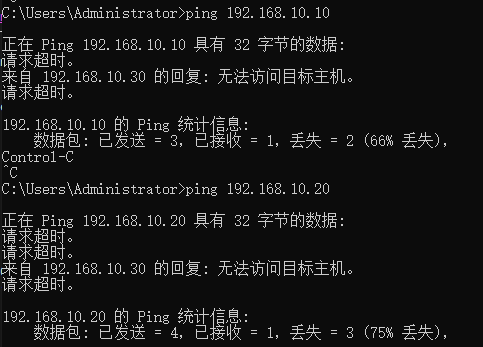
\includegraphics{img/pc3_ping(1).png}
        }
        \subcaption{PC3不可以ping通PC1、PC2}
    \end{minipage}
    \caption{测试三台主机之间的连通性}
\end{figure}
\end{itemize}

\subsubsection{原因分析}
虽然Trunk端口允许所有VLAN通过，但交换机B上尚未配置VLAN，PC3仍在VLAN 1中，与PC1（VLAN 10）、PC2（VLAN 20）不在同一VLAN。

\subsection{步骤5：在交换机B上创建VLAN 20并划分端口}
\subsubsection{操作内容}
在交换机B上：
\begin{lstlisting}[language=bash]
vlan 20
description technical
quit
interface GigabitEthernet 0/0/5
port link-type access
port default vlan 20
quit
\end{lstlisting}

\subsubsection{预期结果}
\begin{itemize}
    \item \texttt{display vlan 20} 显示端口5已加入VLAN 20。
     \begin{figure}[H]
    \centering
    \adjustbox{
        max width=0.8\linewidth,
        max height=0.6\textheight,
        min width=1cm,
        min height=1cm,
        keepaspectratio
    }{
        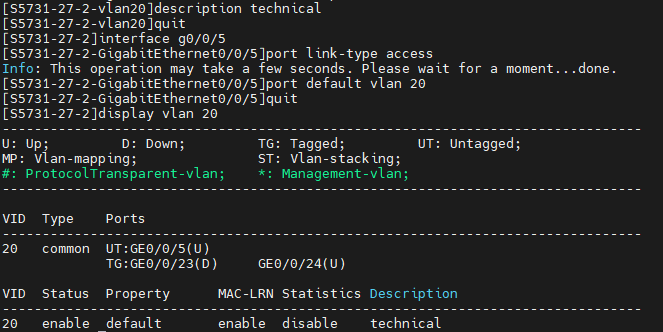
\includegraphics{img/vlan20(1).png}
    }
    \caption{成功划分交换机B的端口5到VLAN20}
     \end{figure}
    \item PC2与PC3可以 ping 通，但不能与PC1ping通；PC1与PC2、PC3无法 ping 通。
     \begin{figure}[H]
    \centering
    % 第一张图片
    \begin{minipage}[t]{0.48\textwidth}
        \centering
        \adjustbox{
            max width=1.05\linewidth,
            max height=0.45\textheight,
            min width=1cm,
            min height=1cm,
            keepaspectratio
        }{
            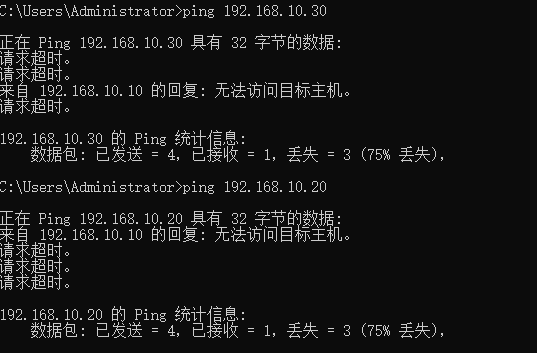
\includegraphics{img/pc1_ping(1).png}
        }
        \subcaption{PC1不可以ping通PC2、PC3}
    \end{minipage}
    \hfill
    % 第二张图片
    \begin{minipage}[t]{0.48\textwidth}
        \centering
        \adjustbox{
            max width=1\linewidth,
            max height=0.45\textheight,
            min width=1cm,
            min height=1cm,
            keepaspectratio
        }{
            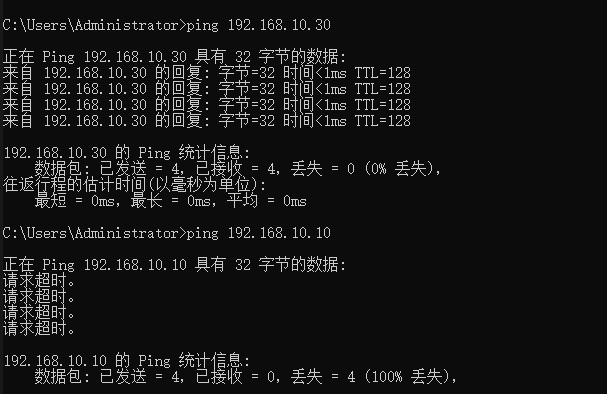
\includegraphics{img/PC2_ping(1).png}
        }
        \subcaption{PC2不可以ping通PC1,可以ping通PC3}
        \end{minipage}
    \end{figure}
\end{itemize}

\subsubsection{原因分析}
PC2和PC3同属VLAN 20，且交换机间Trunk链路允许VLAN 20通过，因此可以通信。PC1在VLAN 10，与VLAN 20隔离。

\subsection{步骤6：配置交换机B与交换机A之间的Trunk链路}
\subsubsection{操作内容}
在交换机B上：
\begin{lstlisting}[language=bash]
interface GigabitEthernet 0/0/24
port link-type trunk
port trunk allow-pass vlan all
quit
\end{lstlisting}

\subsubsection{实验结果}
PC2与PC3可通信，PC1与PC3不可通信。
\begin{figure}[H]
    \centering
    \adjustbox{
        max width=0.8\linewidth,
        max height=0.6\textheight,
        min width=1cm,
        min height=1cm,
        keepaspectratio
    }{
        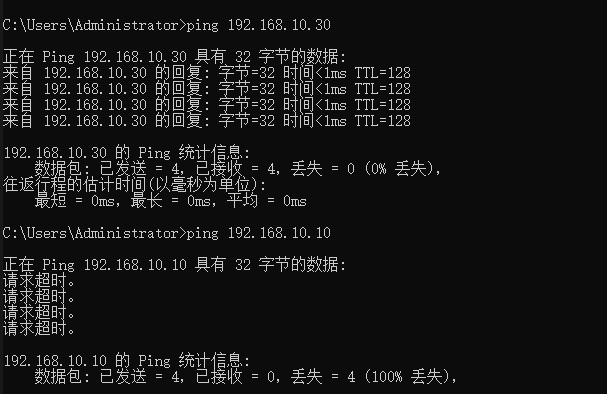
\includegraphics{img/PC2_ping(1).png}
    }
    \caption{PC2不可以ping通PC1,可以ping通PC3}
     \end{figure}
\subsubsection{原因分析}
两台交换机之间的Trunk链路已建立，允许所有VLAN通过。PC2和PC3同属VLAN 20，可跨交换机通信；PC1在VLAN 10，与VLAN 20隔离。

\newpage
\section{拓展实验}
\subsection{实验内容与拓扑结构}
实验网络采用分层设计，分为弱电箱区域和客厅区域两个主要部分：

\begin{figure}[H]
    \centering
    \adjustbox{
        max width=0.8\linewidth,
        max height=0.6\textheight,
        min width=1cm,
        min height=1cm,
        keepaspectratio
    }{
        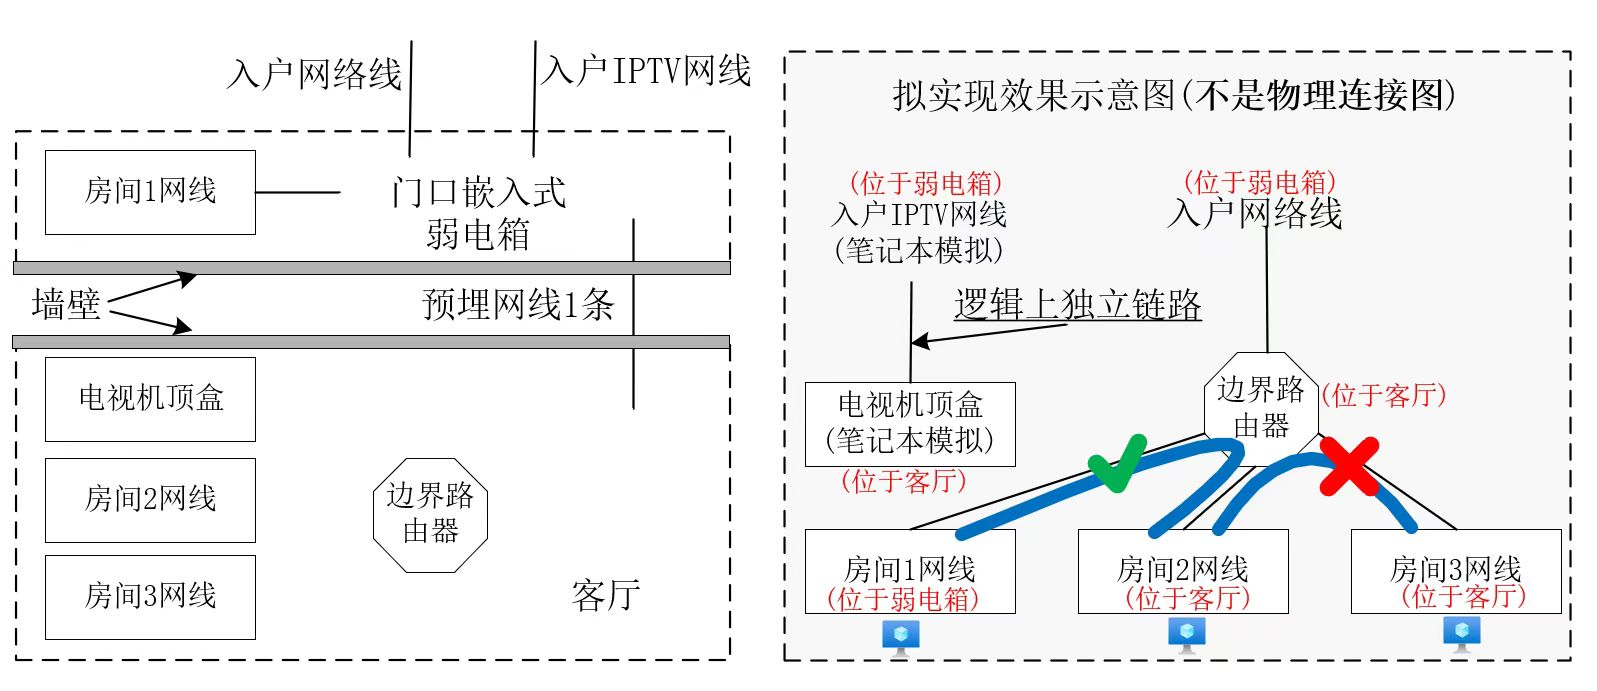
\includegraphics{img/tuozhan.jpg}
    }
    \caption{拓展实验网络拓扑图}
\end{figure}

\textbf{实验要求}
\begin{itemize}
    \item 拟实现右侧效果，请根据左侧内容提供物理连接图，如果需要补充设备，请自行决定，并阐述物理连接图的工作原理。
    \item 根据连接图，利用实验室设备尝试实现。其中，可用笔记本充当IPTV源、另一个笔记本充当电视机顶盒，能ping通即可。房间以PC代表。
    \item 请在实验报告中给出相应的证明截图、配置命令及说明。
\end{itemize}

\begin{table}[H]
\centering
\begin{tabular}{|c|c|c|}
\hline
\textbf{区域} & \textbf{设备} & \textbf{功能描述} \\
\hline
弱电箱区域 & S1交换机 & 核心交换设备，连接所有入户口设备 \\
\hline
客厅区域 & S2边界路由器 & 三层交换设备，实现VLAN间路由 \\
\hline
\end{tabular}
\caption{网络拓扑分区说明}
\end{table}

\subsection{实验设计}
\subsubsection{基本网络访问要求}
\begin{enumerate}
    \item \textbf{互联网访问}：PC1、PC2、PC3均可正常访问互联网（L1）
    \item \textbf{房间间通信}：PC1与PC2之间可以相互通信，PC2与PC3之间不可以互相通信
    \item \textbf{业务专用通信}：机顶盒L3可以访问IPTV源L2
    \item \textbf{跨区域路由}：通过S2实现VLAN间路由功能
\end{enumerate}

\subsubsection{VLAN划分方案:基于业务类型划分}
\begin{itemize}
    \item \textbf{VLAN 10 - 普通用户业务}：
    \begin{itemize}
        \item \textbf{业务成员：} PC1（用户终端）、PC2（用户终端）、L1（网络源/互联网出口）
        \item \textbf{业务逻辑：}这个VLAN专门用于承载普通的互联网数据流量。所有需要上网的设备（PC1, PC2, PC3）其数据流的目的地都是L1。将PC1和L1放在同一个VLAN内，它们之间的通信是二层交换，效率最高。PC3虽然IP网段不同，但通过S2的三层路由功能，也能高效地访问L1。
    \end{itemize}
    \item \textbf{VLAN 20 - 高级用户业务}：包含PC3，禁止与VLAN 10通信
    \item \textbf{VLAN 30 - IPTV业务}：包含IPTV源L2和机顶盒L3，允许相互通信 
    \begin{itemize}
        \item \textbf{业务成员：} L2（IPTV视频源）、L3（机顶盒）
        \item \textbf{业务逻辑：} 这个VLAN是专门的视频流量通道。IPTV流量通常需要较高的服务质量和稳定性，避免被普通数据流量（如下载、游戏）干扰。将视频源（L2）和接收端（L3）放在一个独立的VLAN中，相当于为视频数据建立了一条“专用高速公路”，与“普通公路”（VLAN 10）隔离开。
    \end{itemize}
\end{itemize}

\subsubsection{拓扑图设计}
\begin{figure}[H]
    \centering
    \adjustbox{
        max width=0.8\linewidth,
        max height=0.6\textheight,
        min width=1cm,
        min height=1cm,
        keepaspectratio
    }{
        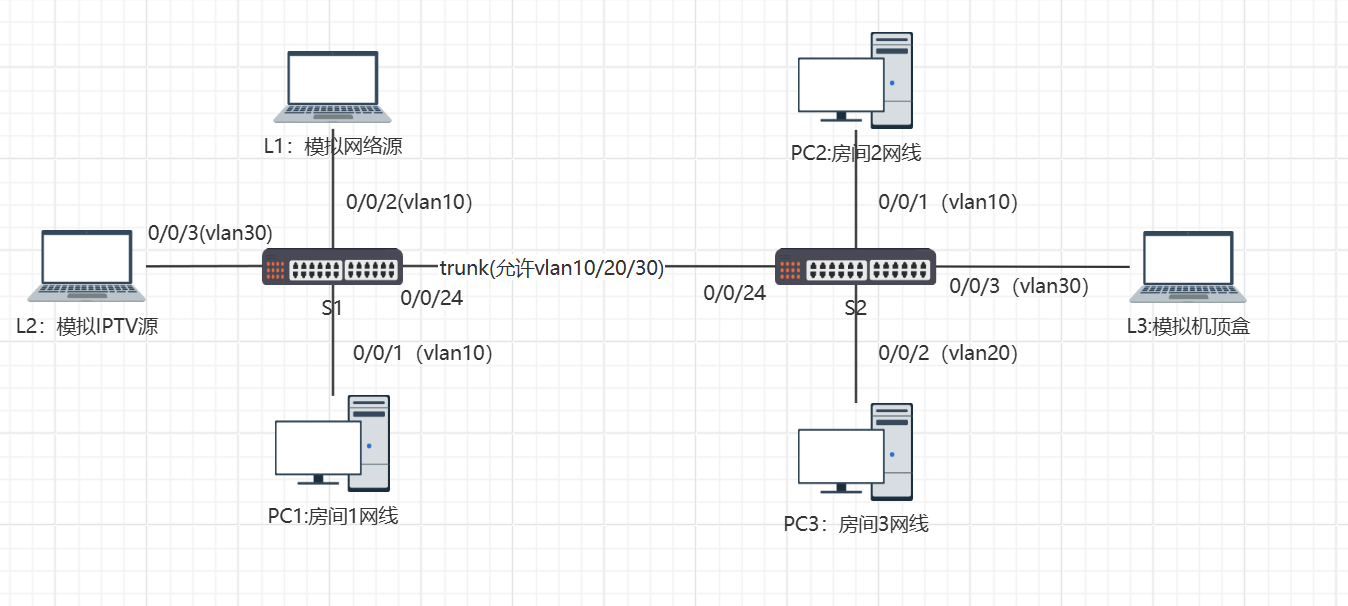
\includegraphics{img/tuopu_1.png}
    }
    \caption{拓展实验网络拓扑图}
\end{figure}

\subsubsection{物理连接关系}
\begin{itemize}
    \item \textbf{弱电箱区域（S1交换机）}：
    \begin{itemize}
        \item 连接入户网络线（笔记本L1模拟网络源）
        \item 连接入户IPTV网线（笔记本L2模拟IPTV源）
        \item 连接房间1网线（PC1）
        \item 通过预埋网线连接至客厅S2设备
    \end{itemize}
    
    \item \textbf{客厅区域（S2边界路由器）}：
    \begin{itemize}
        \item 连接房间2网线（PC2）
        \item 连接房间3网线（PC3）
        \item 连接电视机顶盒（笔记本L3模拟）
        \item 通过预埋网线与弱电箱S1连接
    \end{itemize}
\end{itemize}

\subsubsection{实验设备详细配置}
\begin{table}[H]
\centering

\begin{tabular}{|c|c|c|c|c|c|}
\hline
\textbf{设备名称} & \textbf{物理位置} & \textbf{模拟角色} & \textbf{IP地址} & \textbf{子网掩码} & \textbf{网关} \\
\hline
L1（笔记本） & 弱电箱 & 网络源 & 192.168.10.100 & 255.255.255.0 & 192.168.10.1 \\
\hline
L2（笔记本） & 弱电箱 & IPTV源 & 192.168.30.100 & 255.255.255.0 & 192.168.30.1 \\
\hline
L3（笔记本） & 客厅 & 机顶盒 & 192.168.30.200 & 255.255.255.0 & 192.168.30.1 \\
\hline
PC1 & 房间1 & 用户终端1 & 192.168.10.10 & 255.255.255.0 & 192.168.10.1 \\
\hline
PC2 & 房间2 & 用户终端2 & 192.168.10.20 & 255.255.255.0 & 192.168.10.1 \\
\hline
PC3 & 房间3 & 用户终端3 & 192.168.20.30 & 255.255.255.0 & 192.168.20.1 \\
\hline
S1 & 弱电箱 & 核心交换机 & 172.16.27.201 & - & - \\
\hline
S2 & 客厅 & 边界路由器 & 172.16.27.202 & - & - \\
\hline
\end{tabular}
\caption{实验设备详细配置表}
\end{table}

\subsection{实验步骤及结果展示}
\subsubsection{配置ip地址}
\begin{figure}[H]
    \centering
    % 第一张图片
    \begin{minipage}[t]{0.8\textwidth}
        \centering
        \adjustbox{
            max width=0.8\linewidth,
            max height=0.3\textheight,
            min width=1cm,
            min height=1cm,
            keepaspectratio
        }{
            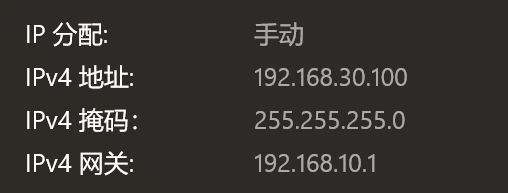
\includegraphics{img/L1.png}
        }
        \subcaption{L1配置}
    \end{minipage}
    
    \vspace{0.5em}
    
    % 第二张图片
    \begin{minipage}[t]{0.8\textwidth}
        \centering
        \adjustbox{
            max width=0.8\linewidth,
            max height=0.3\textheight,
            min width=1cm,
            min height=1cm,
            keepaspectratio
        }{
            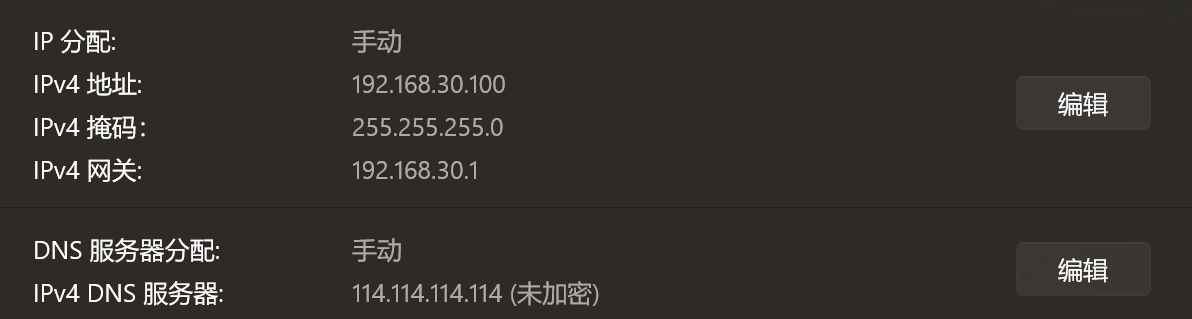
\includegraphics{img/L2.png}
        }
        \subcaption{L2配置}
        \label{fig:pc2-config}
    \end{minipage}
    
    \vspace{0.5em}
    
    % 第三张图片
    \begin{minipage}[t]{0.8\textwidth}
        \centering
        \adjustbox{
            max width=0.8\linewidth,
            max height=0.3\textheight,
            min width=1cm,
            min height=1cm,
            keepaspectratio
        }{
            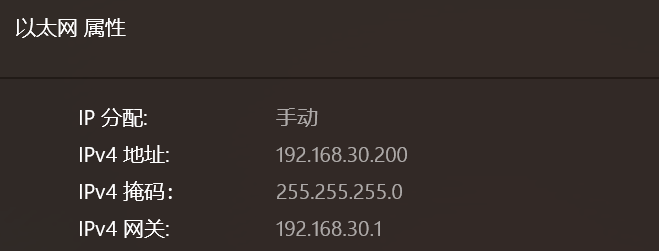
\includegraphics{img/L3.png}
        }
        \subcaption{L3配置}
    \end{minipage}
    \caption{三台笔记本配置}
\end{figure}
三台PC配置同基础实验。
\subsubsection{交换机S1配置}
\begin{lstlisting}[language=bash]
# 登录S1，进入系统视图
system-view
sysname S1

# 创建所需VLAN
vlan batch 10 20 30

# 配置连接终端的端口为Access模式，并划分到相应VLAN
# 假设PC1连接在G0/0/1，L1连接在G0/0/2，L2连接在G0/0/3
interface GigabitEthernet 0/0/1
 port link-type access
 port default vlan 10  # PC1属于数据VLAN

interface GigabitEthernet 0/0/2
 port link-type access
 port default vlan 10  # 网络源L1属于数据VLAN

interface GigabitEthernet 0/0/3
 port link-type access
 port default vlan 30  # IPTV源L2属于IPTV-VLAN

# 配置连接边界路由器S2的端口为Trunk模式
# 假设使用G0/0/24连接S2
interface GigabitEthernet 0/0/24
 port link-type trunk
 port trunk allow-pass vlan 10 20 30  # 允许VLAN 10,20,30的流量通过

quit
save
\end{lstlisting}
\begin{figure}[H]
    \centering
    \adjustbox{
        max width=0.8\linewidth,
        max height=0.6\textheight,
        min width=1cm,
        min height=1cm,
        keepaspectratio
    }{
        
\includegraphics{img/set_s1.png}
    }
    \caption{S1配置截图}
\end{figure}
将PC1和L1放在VLAN10内，将IPTV源L2放在VLAN30内，设置专门视频流量通道。完成配置后，PC1和L1可以ping通，无法ping通L2。

\subsubsection{边界路由器S2配置}

\begin{lstlisting}[caption=S2边界路由器完整配置, language=bash]
# 进入系统视图
system-view

# 设备重命名
sysname S2

# 创建VLAN
vlan batch 10 20 30

# 配置接入端口
interface GigabitEthernet 0/0/1    # PC2
 port link-type access
 port default vlan 10
 description Connect-to-PC2

interface GigabitEthernet 0/0/2    # PC3
 port link-type access
 port default vlan 20  
 description Connect-to-PC3

interface GigabitEthernet 0/0/3    # L3（机顶盒）
 port link-type access
 port default vlan 30
 description Connect-to-L3-STB

# 配置Trunk链路（连接S1）
interface GigabitEthernet 0/0/24
 port link-type trunk
 port trunk allow-pass vlan 10 20 30
 description Trunk-to-S1

# 配置VLAN接口（网关）
interface Vlanif 10
 ip address 192.168.10.1 255.255.255.0
 description Gateway-for-VLAN10

interface Vlanif 20
 ip address 192.168.20.1 255.255.255.0
 description Gateway-for-VLAN20

interface Vlanif 30
 ip address 192.168.30.1 255.255.255.0
 description Gateway-for-VLAN30
\end{lstlisting}
\begin{figure}[H]
    \centering
    \begin{minipage}[t]{0.8\textwidth}
        \centering
        \adjustbox{
            max width=0.8\linewidth,
            max height=0.4\textheight,
            min width=1cm,
            min height=1cm,
            keepaspectratio
        }{
            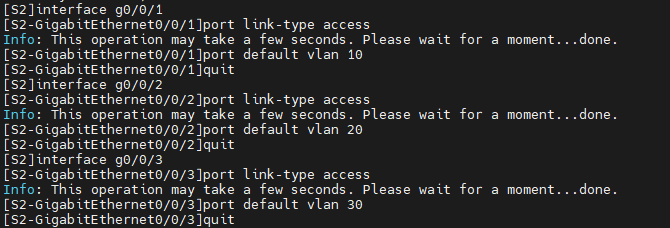
\includegraphics{img/set_s2.png}
        }
    \end{minipage}
    
    \vspace{0.5em}
    
    \begin{minipage}[t]{0.8\textwidth}
        \centering
        \adjustbox{
            max width=0.8\linewidth,
            max height=0.4\textheight,
            min width=1cm,
            min height=1cm,
            keepaspectratio
        }{
            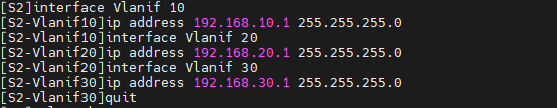
\includegraphics{img/set_s2(1).png}
        }
    \end{minipage}
    \caption{S2配置截图}
\end{figure}
通过配置trunk链路，实现S1与S2之间的多VLAN通信。将PC2放在VLAN10，PC3放在VLAN20，机顶盒L3放在VLAN30。配置VLAN接口作为各VLAN的网关，实现跨VLAN路由。
\subsubsection{ACL访问控制配置}

\begin{lstlisting}[caption=ACL精细化访问控制配置, language=bash]
# 创建高级ACL实现访问控制
acl number 3025
 rule 5 deny ip source 192.168.20.0 0.0.0.255 destination 192.168.10.0 0.0.0.255
 rule 10 deny ip source 192.168.10.0 0.0.0.255 destination 192.168.30.100 0.0.0.0


# 创建流分类
traffic classifier c_isolate operator or
 if-match acl 3025

# 创建流行为
traffic behavior b_isolate
 permit

traffic-filter inbound acl 3025
port link-type trunk
port trunk allow-pass vlan 10 20 30

\end{lstlisting}
通过配置acl，实现对不同VLAN间的访问控制。禁止VLAN20访问VLAN10，禁止VLAN10和VLAN20访问IPTV源L2，确保业务隔离和安全，但允许它们都能访问网关和外部网络。
\begin{figure}[H]
    \centering
    \begin{minipage}[t]{0.8\textwidth}
        \centering
        \adjustbox{
            max width=0.8\linewidth,
            max height=0.4\textheight,
            min width=1cm,
            min height=1cm,
            keepaspectratio
        }{
            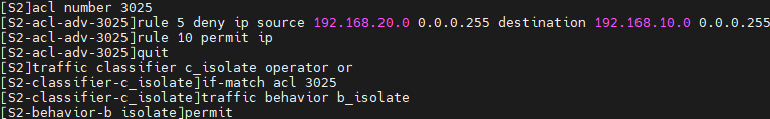
\includegraphics{img/set_acl.png}
        }
    \end{minipage}
    
    \vspace{0.5em}
    
    \begin{minipage}[t]{0.8\textwidth}
        \centering
        \adjustbox{
            max width=0.8\linewidth,
            max height=0.4\textheight,
            min width=1cm,
            min height=1cm,
            keepaspectratio
        }{
            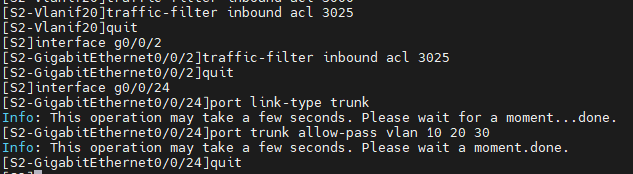
\includegraphics{img/set_acl(1).png}
        }
    \end{minipage}
    \caption{acl截图}
\end{figure}
通过acl设置，实现了PC2与PC3之间的双向通信隔离，保护了IPTV源（L2），禁止普通上网用户（PC1、PC2）访问它。

\subsection{连通性测试结果}
\noindent \textbf{1.首先测试PC1、PC2、PC3之间的连通性：}
    \begin{figure}[H]
    \centering
    % 第一张图片
    \begin{minipage}[t]{0.36\textwidth}
        \centering
        \adjustbox{
            max width=1.05\linewidth,
            max height=0.45\textheight,
            min width=1cm,
            min height=1cm,
            keepaspectratio
        }{
            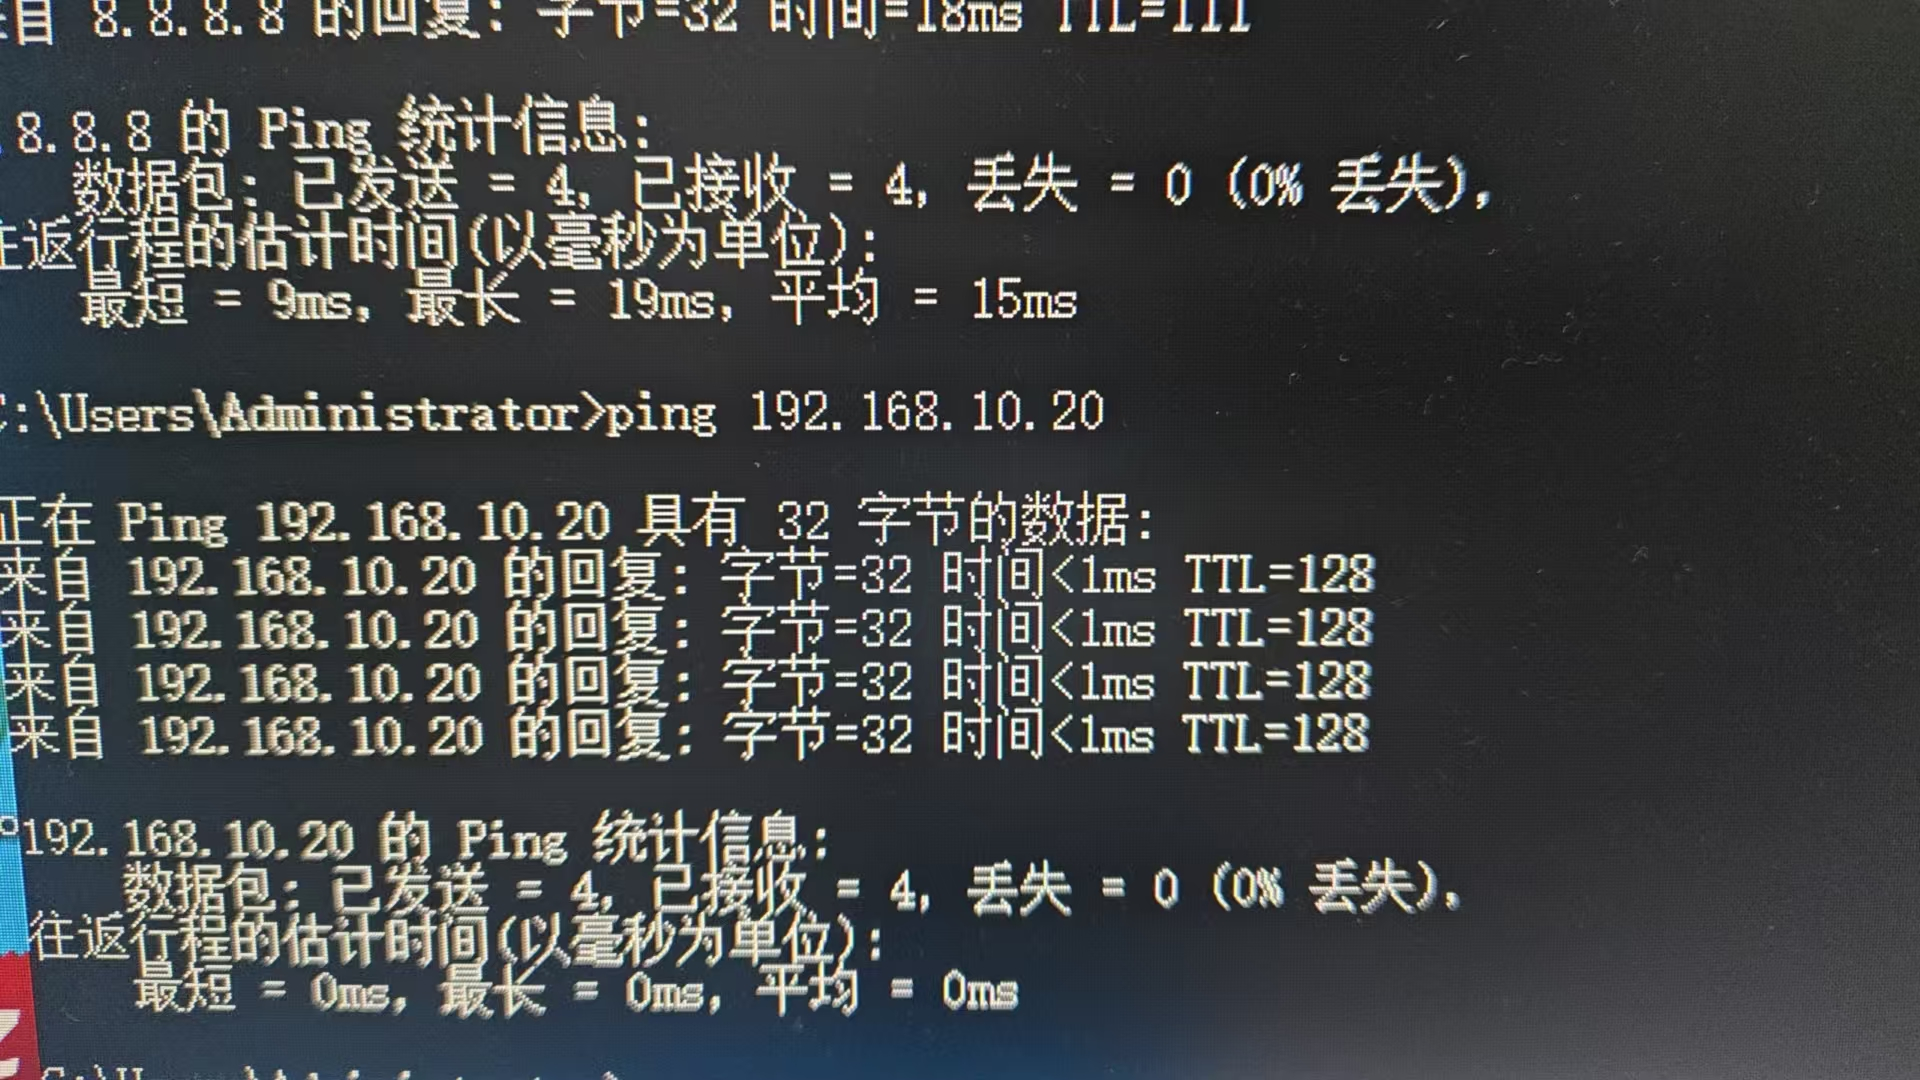
\includegraphics{img/pc1topc2.jpg}
        }
        \subcaption{PC1可以ping通PC2}
    \end{minipage}
    \hfill
    % 第二张图片
    \begin{minipage}[t]{0.6\textwidth}
        \centering
        \adjustbox{
            max width=1\linewidth,
            max height=0.45\textheight,
            min width=1cm,
            min height=1cm,
            keepaspectratio
        }{
            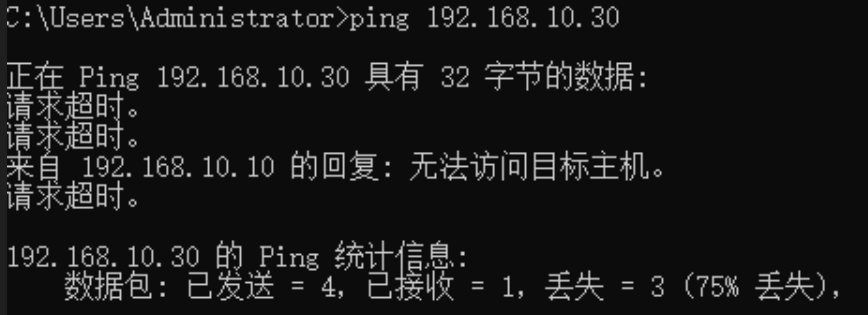
\includegraphics{img/pc2topc3.png}
        }
        \subcaption{PC2不可以ping通PC3}
        \end{minipage}
    \end{figure}
    由于PC1和PC2在VLAN10，PC3在VLAN20，PC1与PC2可以互通，PC2与PC3有ACL隔离，不可以互通。

\vspace{1em}
\noindent \textbf{2.测试机顶盒L3与IPTV源L2的连通性：}
\begin{figure}[H]
    \centering
    \adjustbox{
        max width=0.8\linewidth,
        max height=0.6\textheight,
        min width=1cm,
        min height=1cm,
        keepaspectratio
    }{
        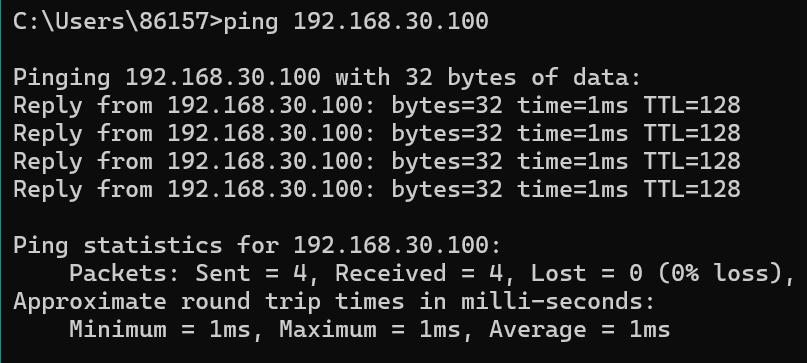
\includegraphics{img/L3pingL2.png}
    }
    \caption{L3可以ping通L2}
\end{figure}
\begin{figure}[H]
由于它们都在VLAN30，且没有ACL限制，可以互通，证明IPTV业务正常。
    \centering
    \adjustbox{
        max width=0.8\linewidth,
        max height=0.6\textheight,
        min width=1cm,
        min height=1cm,
        keepaspectratio
    }{
        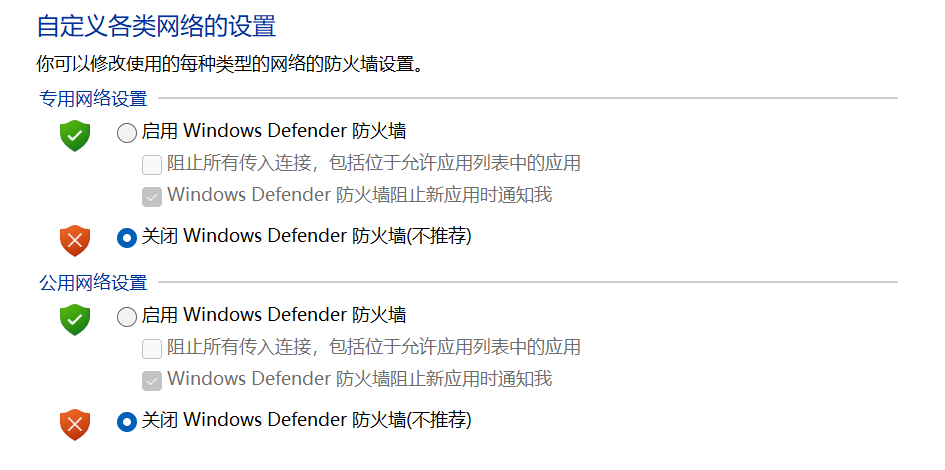
\includegraphics{img/close.png}
    }
    \caption{L2、L3关闭防火墙}
\end{figure}
注意：由于防火墙规则阻止了ICMP协议（即ping命令使用的协议）的请求或回应，必须关闭L2和L3的防火墙，否则ping不通。

\noindent \textbf{3.测试PC1、PC2、PC3访问互联网（L1）的连通性：}
\begin{figure}[H]
    \centering
    \adjustbox{
        max width=0.8\linewidth,
        max height=0.6\textheight,
        min width=1cm,
        min height=1cm,
        keepaspectratio
    }{
        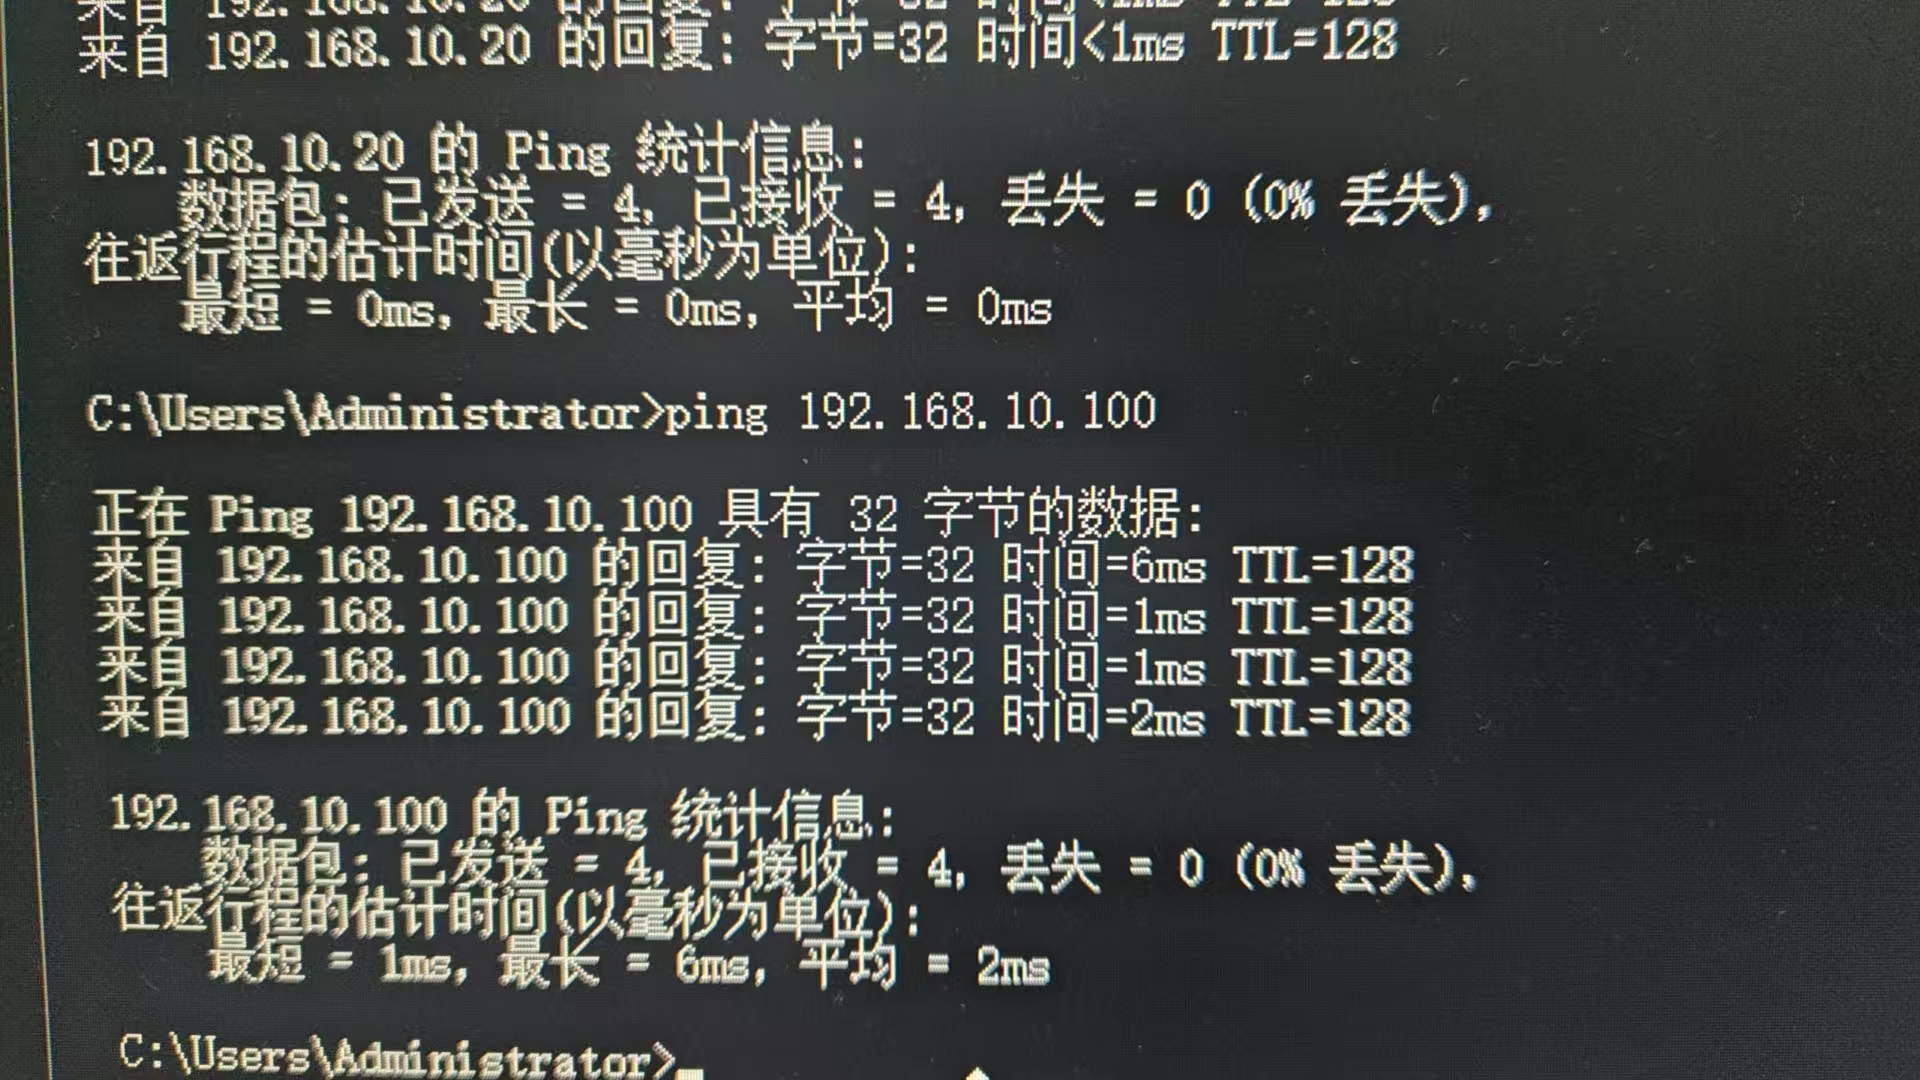
\includegraphics{img/pingL1.jpg}
    }
    \caption{PC1、2、3可访问网络源}
\end{figure}
PC1、PC2、PC3均可以ping通L1，证明它们均能访问互联网(L1是网络源)，满足基本网络访问要求。

\noindent \textbf{4.测试PC1是否联通L2、L3（IPTV隔离是否生效）：}
\begin{figure}[H]
    \centering
    \adjustbox{
        max width=0.8\linewidth,
        max height=0.6\textheight,
        min width=1cm,
        min height=1cm,
        keepaspectratio
    }{
        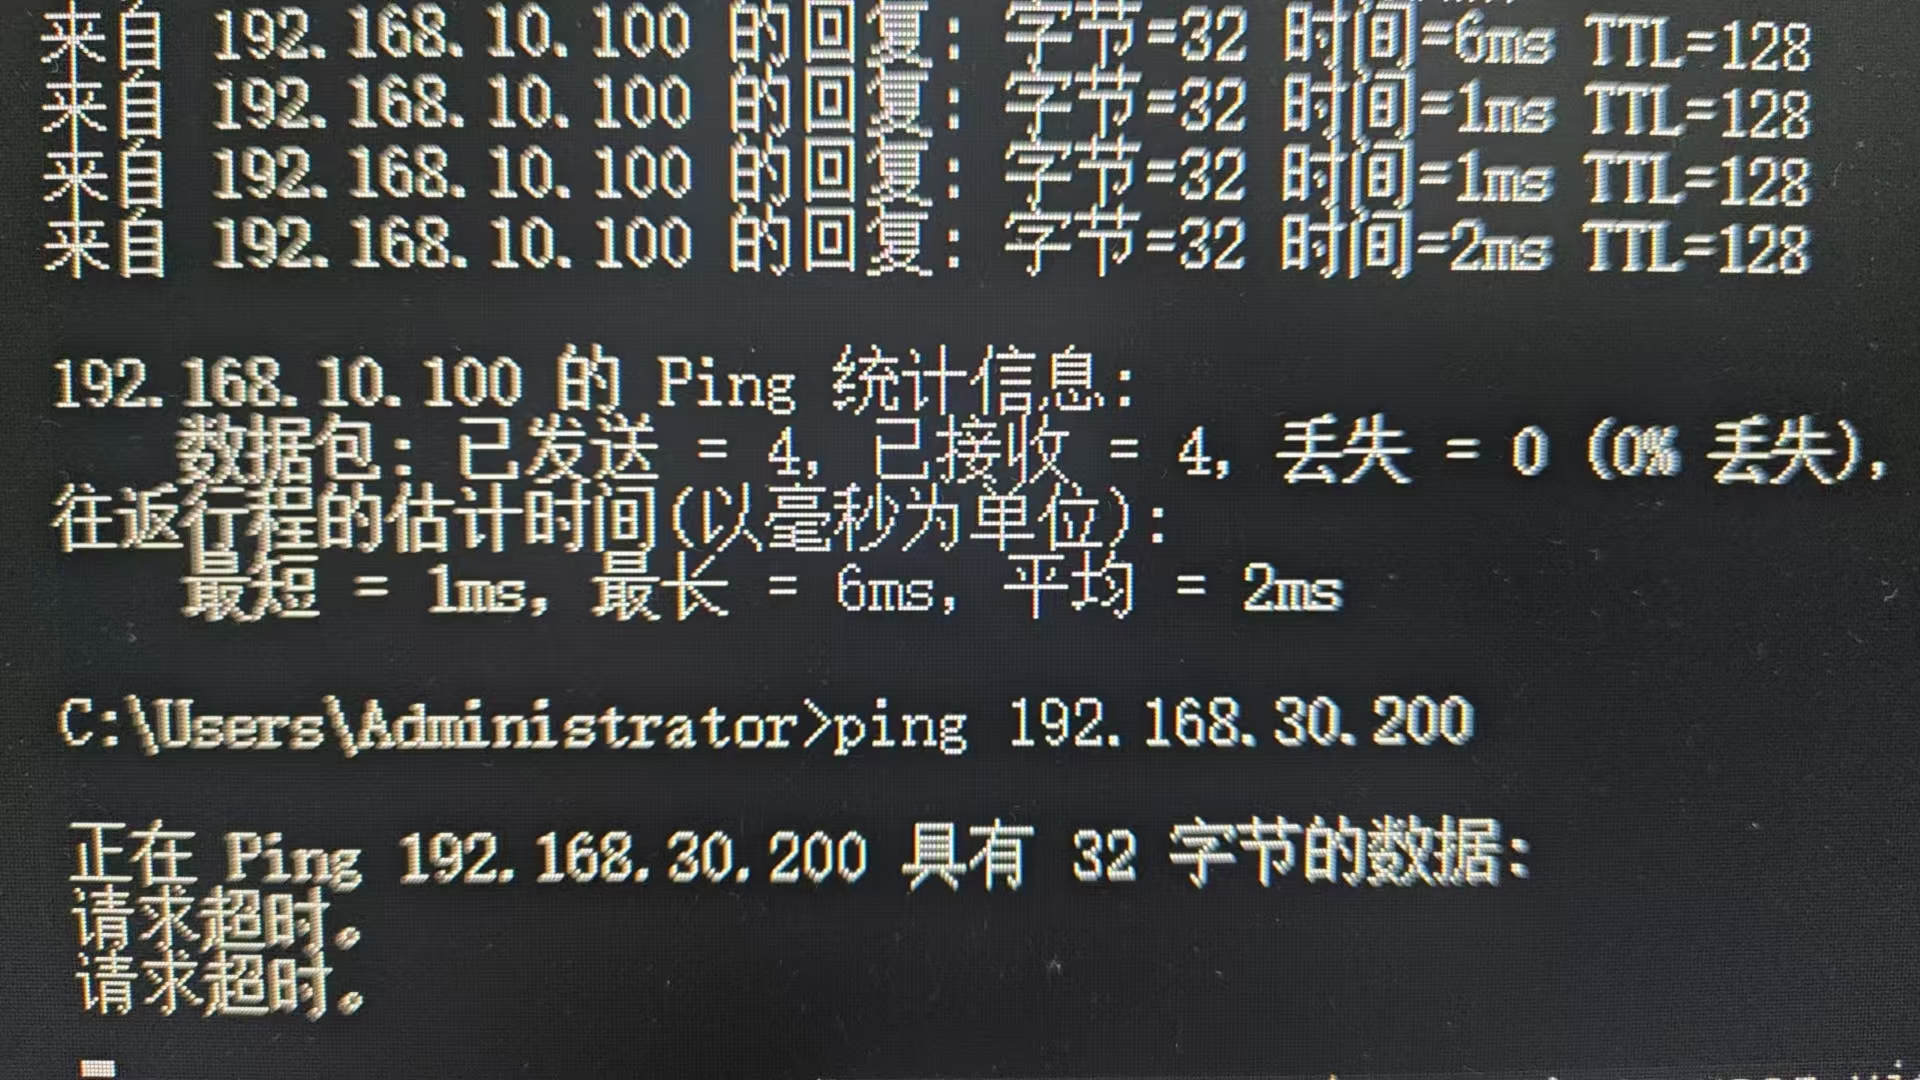
\includegraphics{img/pc1pingl3.jpg}
    }
    \caption{pc1无法ping通L2}
\end{figure}
PC1无法ping通L2和L3，证明IPTV业务隔离生效，普通用户无法访问IPTV源和机顶盒。

\noindent \textbf{5.连通性测试结果总结：}
\begin{table}[H]
\centering
\caption{网络连通性测试结果}
\begin{tabular}{|c|c|c|c|c|c|c|}
\hline
\textbf{源设备} & \textbf{目标设备} & \textbf{预期结果} & \textbf{实际结果} & \textbf{是否符合} & \textbf{测试命令} & \textbf{说明} \\ 
\hline
PC1 & PC2 & 通 & 通 & 符合预期 & ping 192.168.10.20 & 同VLAN通信 \\ 
\hline
PC2 & PC3 & 不通 & 不通 & 符合预期 & ping 192.168.20.30 & ACL隔离生效 \\ 
\hline
PC1、2、3 & L1 & 通 & 通 & 符合预期 & ping 192.168.10.100 & 上网权限验证 \\ 
\hline
L3 & L2 & 通 & 通 & 符合预期 & ping 192.168.30.100 & IPTV业务正常 \\ 
\hline
PC1 & L2 & 不通 & 不通 & 符合预期 & ping 192.168.30.100 & IPTV隔离生效 \\ 
\hline
\end{tabular}
\end{table}

\vspace{2em}
\section{总结与体会}
通过本次VLAN实验，我们深入理解了虚拟局域网的概念及其在网络隔离和管理中的重要作用。实验过程中，我们成功配置了多个VLAN，实现了不同业务之间的隔离，确保了网络的安全性和性能。

在基础实验中，我们通过划分VLAN，验证了不同VLAN间的通信隔离效果，理解了Trunk链路的配置及其在多VLAN环境中的作用。拓展实验进一步加深了我们对VLAN应用的理解，通过实际配置和测试，掌握了如何利用VLAN实现复杂的网络需求，如业务隔离和跨VLAN路由。

此外，实验过程中遇到的各种问题，如ACL配置、端口模式设置等，也锻炼了我们的实际操作能力和问题解决能力。通过查阅资料和反复调试，我们成功解决了问题。
\end{document}